\section{Tablets}
\label{section:tablets}

\subsection{Variante A: Feste Tablets}
\subsubsection{Beschreibung}
Hier geht es um Tablets, die auf einer Halterung montiert sind, und auf dem Weg, den die Mitarbeiter täglich begehen (z.B. Weg zur Stechuhr oder Kantine), positioniert sind. Die Mitarbeiter sollen dazu motiviert werden, aus Eigeninitiative die Umfrage auszufüllen. Die Authentisierung der Mitarbeiter müsste entweder durch einen Login oder einen Stempelkartenleser realisiert werden. Wahrscheinlich müsste dazu zu Beginn der Aktion eine aufwändige Werbemaßnahme durchgeführt werden, um das Interesse der Mitarbeiter auf die Tablets zu lenken. Außerdem muss auf den Tablets ein Guided Access eingerichtet, die Tablets diebstahlsicher montiert und eine permanente Stromversorgung eingerichtet werden. Des Weiteren ist eine regelmäßige Kontrolle der Funktionstüchtigkeit (z.B. einmal am Tag) und es sind gegebenenfalls Wartungsarbeiten und Instandsetzungsmaßnahmen nötig.

\subsubsection{Mockups}
 
\begin{figure}[H]
\centering
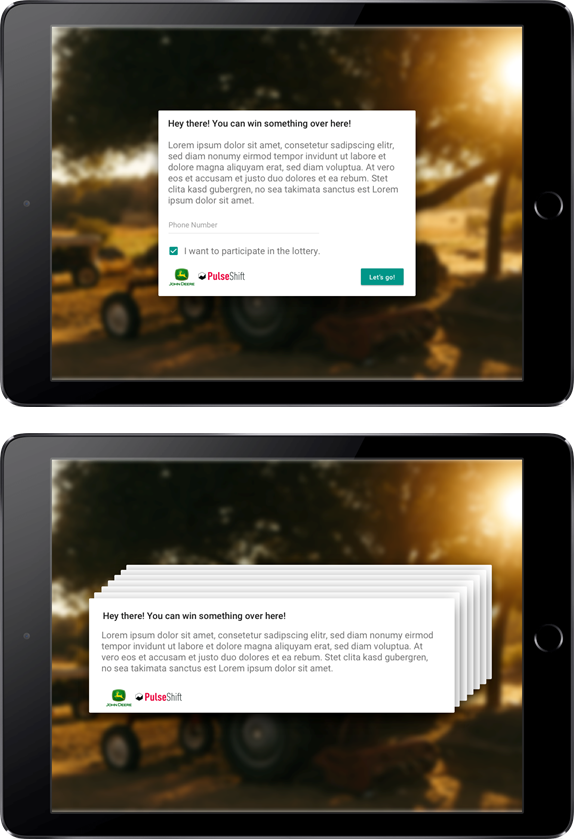
\includegraphics[width=0.7\textwidth]{images/portfolio/tablets}
\caption[Mockup Tablets]{Mockup Tablets}
\label{fig:portfolio:tablets}
\end{figure}
 
\subsubsection{Kostenfaktoren}

\paragraph{Initiale Kosten}
Die initialen Kosten pro Tablet sind im Folgenden angegeben. Mitarbeiter laufen in der Regel in Gruppen (z.B. Schichtende/Mittagspause) an diesem statisch platzierten Tablets vorbei. Da sie nicht für eine Umfrage anstehen und warten möchten, ist eine größere Anzahl Tablets nötig, um eine hohe Beteiligung zu erhalten.

\begin{itemize}
\item Tablet (z.B. Amazon Fire HD 8: 90 €)
\item Ständer (z.B. 90 €)
\item Stromversorgung (z.B. 10 €)
\item Montage (z.B. 50 €)
\end{itemize}

Dies ergibt 240 € pro Tablet.

\paragraph{Regelmäßige Kosten}
\begin{itemize}
\item Tägliches Überprüfen der Funktionstüchtigkeit: Dies dauert ca. 5 min/Stück und kann durch eine gering qualifizierte Kraft (Lohn: 10 €/h) wie z.B. einen Mitarbeiter auf 450 € Basis durchgeführt werden. Somit sind dies pro Tablet und Tag zwischen 80 und 90 ct.
\item Reparaturmaßnahmen: Dieser Aufwand ist in der Theorie schwer schätzbar und müsste durch praktische Tests verifiziert werden. Wir sind von 1 h/Tablet und Monat ausgegangen. Die Maßnahmen müssten durch eine höher qualifizierte Kraft (Lohn: 20 €/h) durchgeführt werden. Dies würde 20 €/Tablet und Monat entsprechen. Allerdings besteht hier die Gefahr, dass deutlich höhere Kosten zum Beispiel durch Neuanschaffungen bei Diebstahl nötig sind.
\end{itemize}

Die geschätzten Werte würden Kosten von 37 €/Tablet und Monat bedeuten.

\subsubsection{Beurteilung des Projektteams}
\paragraph{Vorteile}

\begin{itemize}
\item Die Umfrage könnte „on the fly“ in den Weg des Mitarbeiters durch das Gebäude integriert werden.
\item Es muss nicht die private Hardware der Mitarbeiter genutzt werden.
\end{itemize}

\paragraph{Nachteile}

\begin{itemize}
\item Es fallen hohe Anschaffungskosten an.
\item Ein Guided Access muss eingerichtet werden.
\item Die Tablets müssen regelmäßig überprüft werden.
\item Es kann zu Bedienungsproblemen kommen, wodurch die Motivation der Mitarbeiter, an der Umfrage teilzunehmen, verringert wird.
\item Es müssen Standortgenehmigungen eingeholt werden. Hier könnte es aufgrund der Thematik Arbeitssicherheit Einschränkungen geben, wo Tablets positioniert werden dürfen.
\item Da sich der Mitarbeiter aktiv einloggen muss, wird ihm vor Augen geführt, dass er nicht anonym ist. Dies könnte eine nicht wahrheitsgemäße Beantwortung der Fragen zur Folge haben.
\item Es ist fraglich, ob ein repräsentatives Umfrageergebnis erzielt werden kann, da die Mitarbeiter proaktiv die Umfrage starten müssen und deshalb möglicherweise nicht ausreichend Mitarbeiter teilnehmen.
\item Da die genaue Identität des Mitarbeiters bekannt ist, ist der Kanal datenschutzrechtlich kritisch.
\end{itemize}

\paragraph{Bewertung und Potential}

Der Kanal \glqq Feste Tablets \grqq ist teuer. Außerdem ist der Aufwand, der durch das Verwenden von Hardware erzeugt wird, hoch. So muss zu Beginn die Hardware montiert und regelmäßig überprüft werden. Außerdem muss ein Guided Access auf allen Tablets eingerichtet werden. Die große Anzahl an Nachteilen lässt sich nicht durch die wenigen Vorteile ausgleichen. Somit ist der Kanal \glqq Feste Tablets\grqq in dieser Form für das Anliegen von PulseShift ungeeignet.

\subsection{Variante B: Fragesteller mit Tablet}
\subsubsection{Beschreibung}
Hier geht es um Fragesteller, die sich durch die Firmengebäude bewegen und aktiv Mitarbeiter ansprechen. Die Umfrageergebnisse werden auf dem Tablet z.B. in einer Webapp festgehalten. Die Authentisierung der Mitarbeiter könnte durch allgemeine Fragen (z.B. in welcher Abteilung arbeiten Sie) oder den Ort, an dem der Interviewer den Mitarbeiter angetroffen hat, vorgenommen werden. Somit würde keine genaue Feststellung der Identität vorgenommen, die datenschutzrechtlich kritisch wäre. Der Fragesteller wird speziell für den Umgang mit dem Tablet geschult. Da die Tablets nicht dem direkten Einfluss der Mitarbeiter ausgesetzt sind, sondern von einer geschulten Kraft bedient werden, wird die Ausfall- und Diebstahlrate wahrscheinlich reduziert sind. Die Kontrolle der Funktionstüchtigkeit kann unmittelbar vom Fragesteller durchgeführt werden.

\subsubsection{Kostenfaktoren}

\paragraph{Initiale Kosten}
Die initialen Kosten pro Tablet sind im Folgenden angegeben. Da die Umfrage während der gesamten Arbeitszeit durchgeführt wird und nicht zum Beispiel auf Schichtwechsel eingeschränkt ist, sind weniger Tablets als in Variante A nötig.

\begin{itemize}
\item Tablet (z.B. Amazon Fire HD 8: 90 €)
\item Einstellen und Schulen des Fragestellers (z.B. 100 €)
\end{itemize}

Dies ergibt 190 € pro Tablet.

\paragraph{Regelmäßige Kosten}

\begin{itemize}
\item Betreuung der Umfrage: ca. 6 min/Umfrage. Die kann durch eine gering qualifizierte Kraft wie z.B. einen 450€ Jobber (10€/h) durchgeführt werden. Dies entspricht 1 €/Umfrage.
\item Reparaturmaßnahmen: Die Kosten sind geringer als bei Variante A, da das Tablet nicht dem Einfluss vieler, sondern nur dem Einfluss des Fragestellers ausgesetzt ist. Wir sind von 0,5 h/Tablet und Monat ausgegangen. Die Maßnahmen müssten durch eine höher qualifizierte Kraft (Lohn: 20 €/h) durchgeführt werden. Dies würde 10 €/Tablet und Monat entsprechen. Allerdings besteht hier die Gefahr, dass deutlich höhere Kosten zum Beispiel durch Neuanschaffungen bei Diebstahl nötig sind.
\end{itemize}

Die geschätzten Werte würden Kosten von 10€/Tablet und Monat sowie 1€/Umfrage bedeuten.

\subsubsection{Beurteilung des Projektteams}
\paragraph{Vorteile}

\begin{itemize}
\item Mitarbeiter können durch den Fragesteller aktiv ausgewählt werden.
\item Mitarbeiter werden aktiv angesprochen. Somit ist keine Eigeninitiative nötig,
\item Die Qualität der Antworten kann durch die persönliche Befragung gesteigert werden,
\item Es muss kein Guided Access eingerichtet werden, da der Fragesteller speziell geschult wird.
\item Es muss nicht die private Hardware der Mitarbeiter genutzt werden.
\end{itemize}

\paragraph{Nachteile}

\begin{itemize}
\item Die regelmäßigen Kosten sind insbesondere mit 1 €/Umfrage sehr hoch.
\item Eine Skalierung wäre sehr teuer.
\item Der Fragesteller muss Zugang zu den Unternehmensgebäuden erhalten.
\item Der Mitarbeiter wird bei der Arbeit unterbrochen.
\end{itemize}

\paragraph{Bewertung und Potential}

Prinzipiell könnte der Ansatz das vielleicht beste Umfrageergebnis erzielen. Die Kosten sind jedoch sehr hoch. Deshalb eignet sich dieser Ansatz nicht.

\subsection{Feedback und Beurteilung durch PulseShift}

\begin{itemize}
\item PulseShift konnte in Erfahrung bringen, dass es Tabletlösungen in Form von Terminals (Verschiebbares Tablet in Fassung) in Unternehmen bereits gibt. Dies lässt darauf schließen, dass die Kosten für Unternehmen grundsätzlich nicht zu hoch sind.
\item Für feste Installationen müssen Hotspots gefunden werden, an denen möglichst viele Mitarbeiter vorbei kommen.
\item Eine Kooperation mit externen Dienstleistern wie zum Beispiel iFeedback kommt für PulseShift eher nicht in Frage, da die Überschneidungen zu hoch sind.
\end{itemize}

\subsection{Weiteres Vorgehen}

Das Projektteam und PulseShift sind sich einig, dass Tablets grundsätzlich ein vielversprechender Umfragekanal sind. Allerdings ist der Aufwand zur Entwicklung einer eigenen Lösung sehr hoch und eine Kooperation mit externen Dienstleistern kommt vorerst nicht in Frage. Es wird nicht als sinnvoll betrachtet, den Umfragekanal Tablets im Rahmen dieses Projekts weiter zu betrachten oder einen \gls{poc} zu erstellen.